Soit $\left(u_n\right)$ la suite définie par $u_0 = - 1$ et, pour tout entier naturel $n$ : \[u_{n+1} = 0,9u_n - 0,3.\]

\begin{enumerate}
	\item 
	\begin{enumerate}
		\item Démontrer par récurrence que, pour tout $n \in \mathbb{N}$, $u_n  = 2 \times 0,9^n - 3$.
		\item En déduire que pour tout $n \in \mathbb{N}$, $- 3 < u_n \leqslant - 1$.
		\item Démontrer que la suite $\left(u_n\right)$ est strictement décroissante.
		\item Démontrer que la suite $\left(u_n\right)$ converge et préciser sa limite.
	\end{enumerate}
	\item On se propose d'étudier la fonction $g$ définie sur $]-3;-1]$ par : \[g(x) = \ln (0,5 x + 1,5) - x.\]
	\begin{enumerate}
		\item Justifier toutes les informations données par le tableau de variations de la fonction $g$ (limites, variations, image de $-1$).
		
		\begin{center}
			\begin{tikzpicture}[double distance=3pt]
				\tkzTabInit[lgt=4]{$x$/1,variations de $g$/2}{$-3$,$-2$,$-1$}
				\tkzTabVar{D-/$-\infty$,+/$g(-2)$,-/$1$}
			\end{tikzpicture}
		\end{center}
		\item En déduire que l'équation $g(x) = 0$ a exactement une solution que l'on notera $\alpha$ et dont on donnera un encadrement d'amplitude $10^{-3}$.
	\end{enumerate}
	\item Dans la suite de l'exercice, on considère la suite $\left(v_n\right)$ définie pour tout $ \in \mathbb{N}$, par : \[v_n = \ln \left(0,5 u_n + 1,5\right).\]
	\begin{enumerate}
		\item En utilisant la formule donnée à la question \textbf{1.(a)}, démontrer que la suite $\left(v_n\right)$ est arithmétique de raison $\ln (0,9)$.
		\item Soit $n$ un entier naturel.
		
		Démontrer que $u_n = v_n$ si, et seulement si $g\left(u_n\right) = 0$.
		\item Démontrer qu'il n'existe aucun rang $k \in \mathbb{N}$ pour lequel $u_k = \alpha$.
		\item En déduire qu'il n'existe aucun rang $k \in \mathbb{N}$ pour lequel $v_k = u_k$.
	\end{enumerate}
\end{enumerate}